\section{Results: Overall Accuracy}

\begin{table}[htbp]
\centering
\caption{Forecast accuracy, validation and test periods}
\label{tab:overall}
\small
\begin{adjustbox}{max width=\textwidth}
\begin{tabular}{lrrrrrr}
\toprule
Model & Valid QLIKE & Test QLIKE & Test MAE ($\times10^{4}$) & Test MSE ($\times10^{8}$) & vs HAR-RV (\%) & vs log-HAR (\%) \\
\midrule
HAR-RV & 0.2606 & 0.2286 & 1.656 & 9.303 & -- & +16.3 \\
log-HAR & 0.2298 & 0.1965 & 1.432 & 8.597 & $-$14.0 & -- \\
HAR-RV-LSTM & 0.2258 & \textbf{0.1935} & \textbf{1.401} & \textbf{8.543} & $-$15.4 & $-$1.6 \\
EGARCH-LSTM & 0.2703 & 0.2709 & 2.034 & 11.856 & +18.5 & +37.8 \\
\midrule
HAR-EGARCH-LSTM & 0.2184 & 0.1931 & 1.444 & 8.703 & $-$15.5 & $-$1.7 \\
\bottomrule
\end{tabular}
\end{adjustbox}
\par\smallskip\parbox{0.95\textwidth}{\footnotesize\itshape Test: 29,774 stock-days, 95 stocks, 1 Jan 2025 -- 9 Apr 2026; validation: 46,599 stock-days, 2023--2024. Last two columns: change in test QLIKE (negative = better). Bold = lowest test loss among the four main models. HAR-EGARCH-LSTM is an ablation.}
\end{table}


\textbf{Ranking.} HAR-RV-LSTM has the lowest test loss on all three measures (Table~\ref{tab:overall},
Figure~\ref{fig:losses}). Its QLIKE of 0.1935 is 15.4\% below HAR-RV and 1.6\% below log-HAR.
EGARCH-LSTM is the weakest model, 18.5\% worse than HAR-RV. The validation ranking is the same.

\textbf{Where the gain over HAR-RV comes from.} log-HAR alone removes 14.0 of the 15.4 points.
Level HAR-RV is pulled up by a few extreme training days and over-forecasts by 21\% on average
(Table~\ref{tab:mz}). The network's own contribution, beyond working in logs, is the remaining 1.6\%.

\begin{figure}[htbp]
\centering
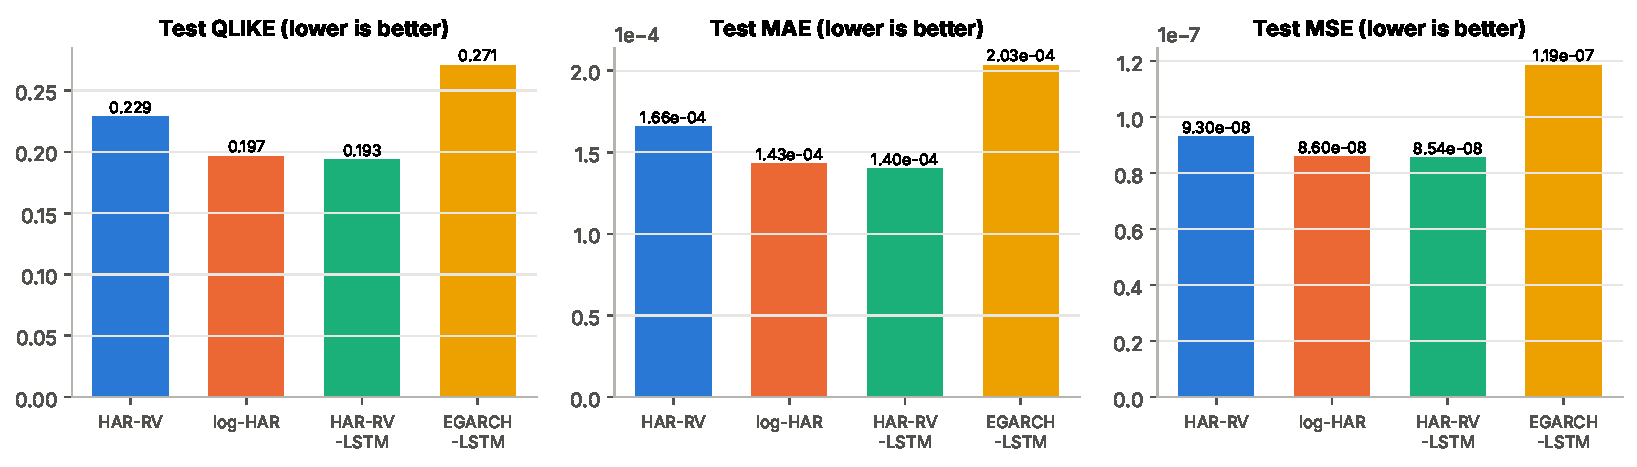
\includegraphics[width=\textwidth]{fig_test_losses.pdf}
\caption{Test-period losses of the four main models (lower is better).}
\label{fig:losses}
\end{figure}

\textbf{Significance.} All differences with HAR-RV are significant (Table~\ref{tab:dm}). HAR-RV-LSTM
against log-HAR: $t=2.80$, Holm $p=0.010$, and the bootstrap interval [0.0011, 0.0054] excludes zero.
On MAE the gain is also significant ($t=4.22$); on MSE it is not ($p=0.26$), because MSE is driven by a
handful of extreme days. Adding EGARCH features to HAR-RV-LSTM changes nothing ($t=0.24$, $p=0.81$).

\begin{table}[htbp]
\centering
\caption{Diebold--Mariano tests on the test period (A vs B)}
\label{tab:dm}
\small
\begin{adjustbox}{max width=\textwidth}
\begin{tabular}{lrrrcrr}
\toprule
Comparison & QLIKE diff (A$-$B) & $t$ & Holm $p$ & 95\% block-bootstrap CI & MAE $t$ & MAE Holm $p$ \\
\midrule
HAR-RV vs log-HAR & 0.0320 & 6.54 & $<$0.001 & [0.0235, 0.0417] & 11.02 & $<$0.001 \\
HAR-RV vs HAR-RV-LSTM & 0.0351 & 6.18 & $<$0.001 & [0.0250, 0.0465] & 10.11 & $<$0.001 \\
log-HAR vs HAR-RV-LSTM & 0.0031 & 2.80 & 0.010 & [0.0011, 0.0054] & 4.22 & $<$0.001 \\
HAR-RV vs EGARCH-LSTM & $-$0.0425 & $-$12.73 & $<$0.001 & [$-$0.0483, $-$0.0359] & $-$9.90 & $<$0.001 \\
log-HAR vs EGARCH-LSTM & $-$0.0745 & $-$10.39 & $<$0.001 & [$-$0.0885, $-$0.0611] & $-$14.90 & $<$0.001 \\
EGARCH-LSTM vs HAR-RV-LSTM & 0.0776 & 9.89 & $<$0.001 & [0.0631, 0.0929] & 14.92 & $<$0.001 \\
HAR-RV-LSTM vs HAR-EGARCH-LSTM & 0.0003 & 0.24 & 0.810 & [$-$0.0016, 0.0027] & $-$5.42 & $<$0.001 \\
\bottomrule
\end{tabular}
\end{adjustbox}
\par\smallskip\parbox{0.95\textwidth}{\footnotesize\itshape Positive difference / $t$ = model B has lower loss. Loss differences averaged across stocks per day (314 days), Newey--West (5 lags) standard errors; Holm adjustment over the seven comparisons per loss. Bootstrap: 5-day blocks, 2,000 draws.}
\end{table}


\textbf{Stability.} The gain builds steadily through the test period rather than coming from a few days
(Figure~\ref{fig:cum}): against log-HAR it is flat until June 2025 and rises after. Each of the three
seeds beats log-HAR on its own (test QLIKE 0.1926--0.1959 against 0.1965; Annex Table~\ref{tab:seeds}).
By stock, HAR-RV-LSTM beats HAR-RV on all 95 stocks and log-HAR on 67 of 95 (70\%).

\begin{figure}[htbp]
\centering
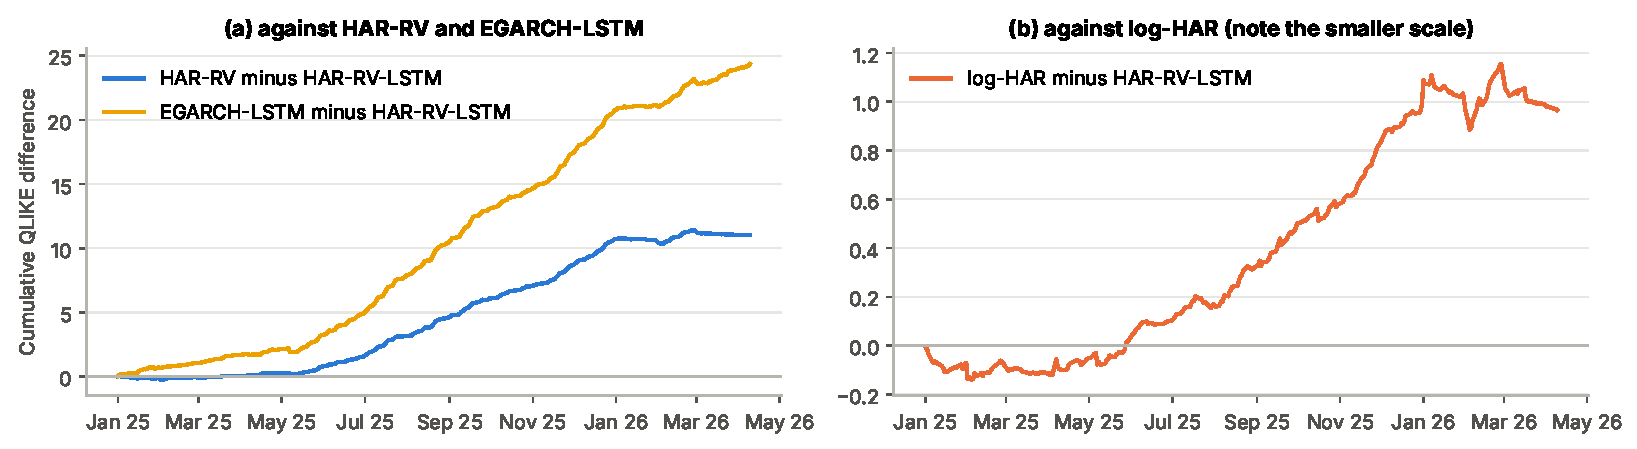
\includegraphics[width=\textwidth]{fig_cumulative_qlike.pdf}
\caption{Cumulative daily QLIKE difference against HAR-RV-LSTM over the test period. A rising line means
HAR-RV-LSTM is ahead.}
\label{fig:cum}
\end{figure}

\begin{figure}[htbp]
\centering
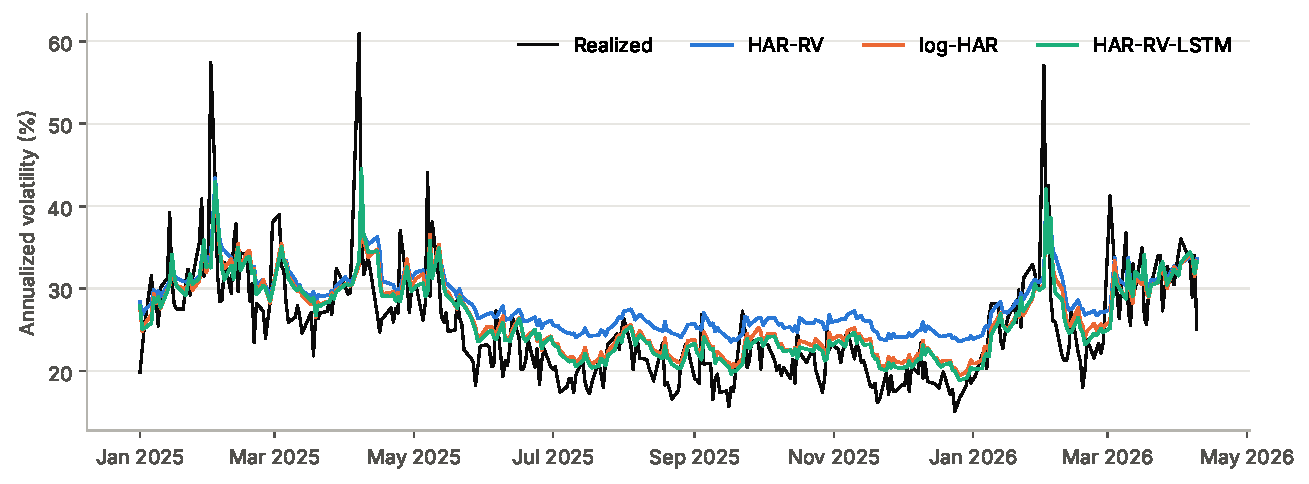
\includegraphics[width=\textwidth]{fig_forecast_vs_actual.pdf}
\caption{Average realized volatility across the 95 stocks and the average forecasts (annualized).}
\label{fig:fva}
\end{figure}

\textbf{Calibration.} HAR-RV sits visibly above realized volatility in the calm second half of 2025
(Figure~\ref{fig:fva}). In Mincer--Zarnowitz regressions HAR-RV-LSTM explains the most variation
($R^2=0.470$ against 0.462 for log-HAR) and has the smallest average bias (6\%).

\begin{table}[htbp]
\centering
\caption{Mincer--Zarnowitz regressions, test period: $\log RV_{t+1}=\alpha+\beta\log\hat h_{t+1}$}
\label{tab:mz}
\small
\begin{adjustbox}{max width=\textwidth}
\begin{tabular}{lrrrrr}
\toprule
Model & $\alpha$ & $\beta$ & s.e.($\beta$) & $R^2$ & Mean forecast / mean RV \\
\midrule
HAR-RV & $-$0.815 & 0.948 & 0.017 & 0.402 & 1.210 \\
log-HAR & $-$0.931 & 0.918 & 0.017 & 0.462 & 1.080 \\
HAR-RV-LSTM & $-$0.775 & 0.934 & 0.018 & 0.470 & 1.059 \\
EGARCH-LSTM & $-$2.193 & 0.790 & 0.014 & 0.348 & 1.395 \\
\bottomrule
\end{tabular}
\end{adjustbox}
\par\smallskip\parbox{0.95\textwidth}{\footnotesize\itshape A well-calibrated forecast has $\beta\approx1$. Standard errors clustered by date.}
\end{table}


\section{Results: Liquidity}

\begin{table}[htbp]
\centering
\caption{Test QLIKE by liquidity group}
\label{tab:liquidity}
\small
\begin{adjustbox}{max width=\textwidth}
\begin{tabular}{lrrrrrrrr}
\toprule
Liquidity & Obs & HAR-RV & log-HAR & HAR-RV-LSTM & EGARCH-LSTM & Gain vs HAR (\%) & Gain vs log-HAR (\%) & DM $t$ \\
\midrule
High & 10,026 & 0.2260 & 0.1920 & \textbf{0.1915} & 0.2477 & 15.3 & 0.3 & 0.38 \\
Medium & 9,716 & 0.2192 & 0.1925 & \textbf{0.1898} & 0.2556 & 13.4 & 1.4 & 2.43 \\
Low & 10,032 & 0.2403 & 0.2050 & \textbf{0.1989} & 0.3087 & 17.2 & 3.0 & 3.96 \\
\bottomrule
\end{tabular}
\end{adjustbox}
\par\smallskip\parbox{0.95\textwidth}{\footnotesize\itshape Gain = percentage reduction in QLIKE of HAR-RV-LSTM. DM $t$: HAR-RV-LSTM against log-HAR within the group (positive = LSTM better). Bold = best model in the group.}
\end{table}


HAR-RV-LSTM is the best model in every liquidity group (Table~\ref{tab:liquidity},
Figure~\ref{fig:liqq}). Its gain over log-HAR rises as liquidity falls: 0.3\% in the most liquid third
(not significant, $t=0.38$), 1.4\% in the middle third ($t=2.43$) and 3.0\% in the least liquid third
($t=3.96$). Across stocks the gain is positively correlated with the illiquidity rank (Spearman 0.29;
Figure~\ref{fig:perstock}). This supports H1: the network helps most where RV is noisiest and a linear
model fits worst. For the most liquid stocks, log-HAR is already as good.

EGARCH-LSTM falls further behind as liquidity falls (QLIKE 0.248 to 0.309): daily returns describe the
volatility of thinly traded stocks particularly poorly.

\begin{figure}[htbp]
\centering
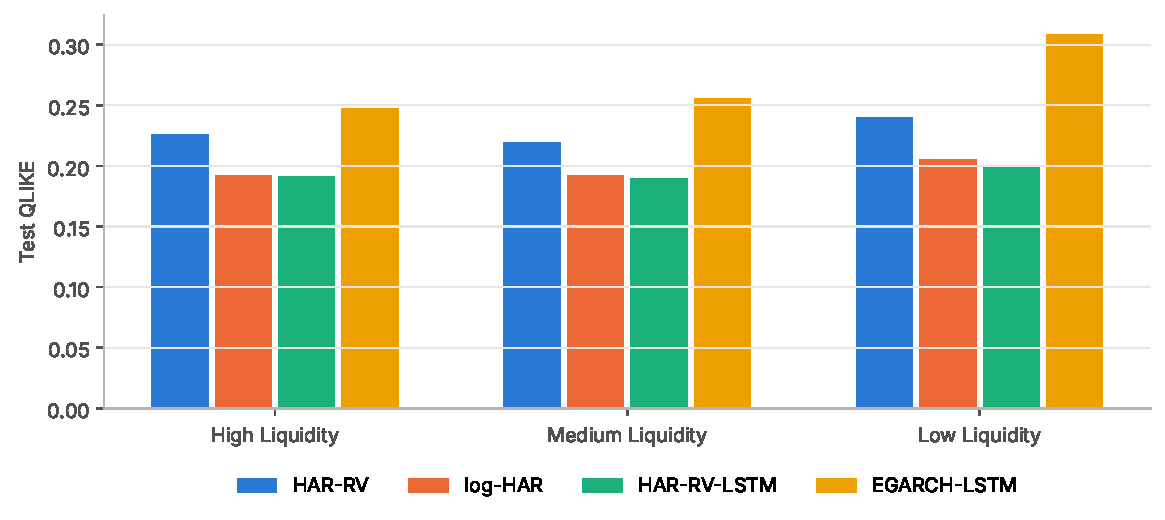
\includegraphics[width=0.85\textwidth]{fig_liquidity_qlike.pdf}
\caption{Test QLIKE by liquidity group.}
\label{fig:liqq}
\end{figure}

\begin{figure}[htbp]
\centering
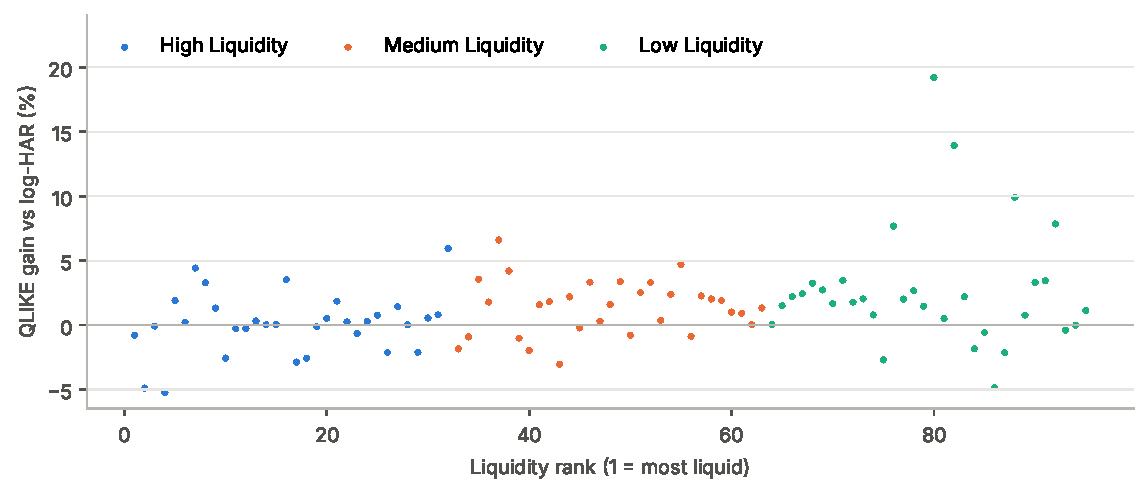
\includegraphics[width=0.85\textwidth]{fig_per_stock_gain.pdf}
\caption{Per-stock QLIKE gain of HAR-RV-LSTM over log-HAR against liquidity rank.}
\label{fig:perstock}
\end{figure}

\section{Results: Market Regimes and Robustness}

\begin{table}[htbp]
\centering
\caption{Test QLIKE by market regime}
\label{tab:regimes}
\small
\begin{adjustbox}{max width=\textwidth}
\begin{tabular}{lrrrrr}
\toprule
Regime & HAR-RV & log-HAR & HAR-RV-LSTM & EGARCH-LSTM & LSTM gain vs log-HAR (\%) \\
\midrule
\multicolumn{6}{l}{\emph{Ex ante: market average RV$_{22}$ on day $t$, training-period terciles}}\\
Calm (253 days) & 0.2344 & 0.1971 & \textbf{0.1936} & 0.2825 & 1.8 \\
Normal (61 days) & 0.2043 & 0.1944 & \textbf{0.1929} & 0.2220 & 0.7 \\
\midrule
\multicolumn{6}{l}{\emph{Ex post: realized RV of the target day, test terciles (descriptive)}}\\
Low RV & 0.3096 & 0.2043 & \textbf{0.1913} & 0.3642 & 6.4 \\
Medium RV & 0.1345 & 0.1043 & \textbf{0.0971} & 0.1814 & 6.8 \\
High RV & \textbf{0.2417} & 0.2810 & 0.2920 & 0.2669 & $-$3.9 \\
\bottomrule
\end{tabular}
\end{adjustbox}
\end{table}


\textbf{Regimes.} Using cut-offs from the training years (which include COVID-19), the test period
contains only calm (253 days) and normal (61 days) markets. The LSTM gains 1.8\% over log-HAR in calm
markets and 0.7\% in normal ones (Table~\ref{tab:regimes}). Sorting by the realized outcome shows the
other side: on the third of days with the highest RV, HAR-RV-LSTM is 3.9\% \emph{worse} than log-HAR,
and HAR-RV is best because it over-forecasts. The LSTM wins on ordinary days and gives some of it back
on spikes, in line with \citet{rahimikia2020}.

\begin{table}[htbp]
\centering
\caption{Test QLIKE in four consecutive sub-periods and without extreme days}
\label{tab:subperiods}
\small
\begin{adjustbox}{max width=\textwidth}
\begin{tabular}{lrrrr}
\toprule
Period & HAR-RV & log-HAR & HAR-RV-LSTM & EGARCH-LSTM \\
\midrule
2025-01-01 -- 2025-04-28 & 0.2048 & \textbf{0.2010} & 0.2018 & 0.2283 \\
2025-04-29 -- 2025-08-19 & 0.2246 & 0.1819 & \textbf{0.1776} & 0.2683 \\
2025-08-20 -- 2025-12-12 & 0.2504 & 0.1891 & \textbf{0.1811} & 0.3003 \\
2025-12-15 -- 2026-04-09 & 0.2351 & 0.2146 & \textbf{0.2136} & 0.2872 \\
\midrule
Full test, top 1\% RV days removed & 0.2053 & 0.1701 & \textbf{0.1662} & 0.2507 \\
\bottomrule
\end{tabular}
\end{adjustbox}
\end{table}


\textbf{Sub-periods and extreme days.} HAR-RV-LSTM is best in three of four sub-periods; in January--April
2025, which includes the April tariff shock, log-HAR is marginally better (0.2010 against 0.2018).
Removing the top 1\% of RV days widens the gain over log-HAR to 2.3\% (Table~\ref{tab:subperiods}).

\begin{figure}[htbp]
\centering
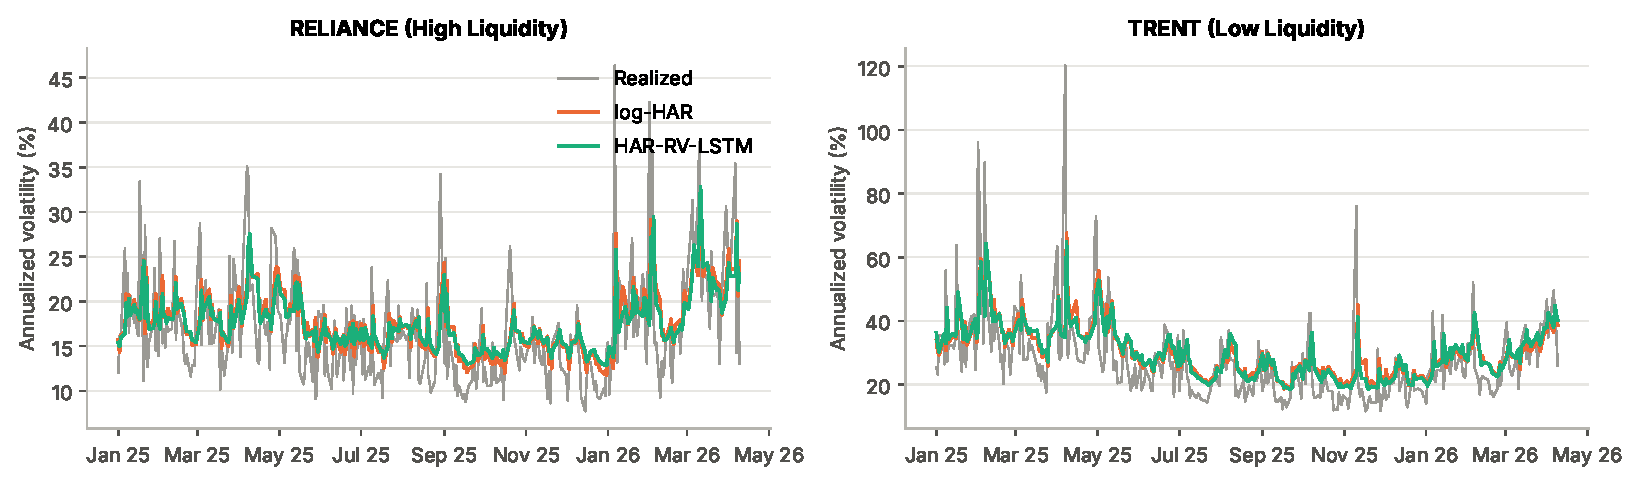
\includegraphics[width=\textwidth]{fig_example_stocks.pdf}
\caption{Realized and forecast volatility for a highly liquid (Reliance) and a less liquid (Trent) stock.}
\label{fig:examples}
\end{figure}

\section{What Changed from the First Version}
\label{sec:versions}

\begin{table}[htbp]
\centering
\caption{Test QLIKE in the first version of the project and after the corrections}
\label{tab:versions}
\small
\begin{adjustbox}{max width=\textwidth}
\begin{tabular}{lrrrr}
\toprule
Model & First version & Corrected & vs HAR-RV, first (\%) & vs HAR-RV, corrected (\%) \\
\midrule
HAR-RV & 0.4230 & 0.2286 & -- & -- \\
HAR-RV-LSTM & 0.3421 & 0.1935 & $-$19.1 & $-$15.4 \\
EGARCH-LSTM & 0.3950 & 0.2709 & $-$6.6 & +18.5 \\
log-HAR & -- & 0.1965 & -- & $-$14.0 \\
\bottomrule
\end{tabular}
\end{adjustbox}
\par\smallskip\parbox{0.95\textwidth}{\footnotesize\itshape First version: 29,830 stock-days, uncleaned RV with overnight gaps, EGARCH fitted on the full sample, liquidity groups from the mis-scaled slope (only 42\% of stocks keep the same group after the correction). The two columns are not on identical samples; compare the relative columns.}
\end{table}


A first version of the project reported a 19.1\% QLIKE gain for HAR-RV-LSTM and a 6.6\% gain for
EGARCH-LSTM over HAR-RV. A code review found three problems:
\begin{enumerate}
\item \textbf{Dirty RV.} RV included the overnight gap and bad prints (VBL on 14 June 2023 jumped from 322
to 644 and back within ten minutes). These spikes inflated level-HAR errors most. Cleaning cut HAR-RV's
test QLIKE from 0.423 to 0.229.
\item \textbf{Liquidity groups.} The slope-based measure divided signed volume by its own mean, which is
close to zero and differs across stocks, so the ranking was close to random (ICICI Bank ``Medium'',
Infosys ``Low''). Only 42\% of stocks keep their group under the corrected Amihud measure.
\item \textbf{EGARCH look-ahead.} EGARCH was estimated on 2016--2026, so its test-period features used
parameters fitted on test data. With training-only parameters, EGARCH-LSTM moves from 6.6\% better to
18.5\% worse than HAR-RV.
\end{enumerate}
The headline survives: HAR-RV-LSTM is still the best model. Its advantage is smaller and better
understood: most of it is the log transformation, and the true network gain is concentrated in less
liquid stocks.
